\documentclass[12pt]{beamer}
\usepackage{xcolor}
\usepackage{pgf,pgfarrows,pgfnodes,pgfautomata,pgfheaps,pgfshade}
\usepackage{algorithm,algorithmic}
\usetheme{Air}

\DeclareMathOperator*{\argmax}{arg\,max}

\title[CSC349A Numerical Analysis]{CSC349A Numerical Analysis}


\logo{\pgfputat{\pgfxy(-0.5,7.5)}{\pgfbox[center,base]{
\includegraphics[width=1.0cm]{figures/uvic}}}}  
\beamertemplatenavigationsymbolsempty

    \defbeamertemplate{footline}{author and page number}{%
      \usebeamercolor[fg]{page number in head/foot}%
      \usebeamerfont{page number in head/foot}%
      \hspace{1em}\insertshortauthor\hfill%
      \insertpagenumber\,/\,\insertpresentationendpage\kern1em\vskip2pt%
    }
    \setbeamertemplate{footline}[author and page number]{}



\subtitle[Lecture 17]{Lecture 17}
\date[2023]{2023}
\author[R. Little]{Rich Little}
\institute[University of Victoria]{University of Victoria}
%\logo{\includegraphics[scale=.25]{unilogo.pdf}}
\begin{document}
\frame{\maketitle} % <-- generate frame with title


\AtBeginSection[]
{
\begin{frame}<beamer>[allowframebreaks]{Table of Contents}
\tableofcontents[currentsection,currentsubsection, 
    hideothersubsections, 
    sectionstyle=show/shaded,
]
\end{frame}
}

\section{Numerical Integration (Quadrature)} 


\begin{frame}{Introduction} 
The process of determining areas e.g. area of a circle by inscribed
and superscribed polygons. This term is used to avoid confusion with
the numeric integration of differential equations.
\\
\noindent 
{\bf Problem:} approximate the value of 
\[
\int_a^{b} f(x) dx
\] 
\noindent 
where $f(x)$ is such that it cannot be integrated analytically or it is known at only a finite set of points. 
\end{frame} 

\begin{frame}{The main idea}
Approximate $f(x)$ by an interpolating polynomial $P(x)$, and approximate $\int_{a}^{b} f(x)dx$ by $\int_a^{b} P(x)dx$
\\
Suppose $P_n(x)$ is the Lagrange form of the interpolating polynomial: 
\[
P_n(x) = \sum_{i=0}^{n} L_i(x) f(x_i)
\]
\noindent 
then 
\[
\int_{a}^{b} f(x)dx \approx \int_{a}^{b} \left [ \sum_{i=0}^{n} L_i(x) f(x_i) \right ] dx = \sum_{i=0}^{n} \left[ \int_a^b L_i(x) dx \right ] f(x_i) 
\]
\noindent 
which is of the form $\sum_{i=0}^{n} a_i f(x_i)$. 
\end{frame} 

\begin{frame}{Quadrature formula} 
So, our approximation is of the form
\[
\int_{a}^{b} f(x)dx \approx \sum_{i=0}^{n} a_i f(x_i).
\]

Such an approximation is called a {\bf quadrature formula}, and $a_i$ are
the {\bf quadrature coefficients} and $x_i$ are the {\bf quadrature points},
the points at which $f(x)$ is sampled to approximate $\int_{a}^{b}
f(x)dx$.

\end{frame} 

\begin{frame}{Types} 
Types of quadrature formulas: 
\begin{itemize} 
\item Newton-Cotes closed 
\item Newton-Cotes open 
\item Gaussian (omit) 
\end{itemize} 

Any quadrature formula derived by integrating an interpolating polynomial at equally-spaced quadrature points is called a {\bf Newton-Cotes} formula. 

{\bf Gaussian formulas} obtain high accuracy by using optimally-chosen, unequally-spaced quadrature points. 
\end{frame}

\begin{frame}{Newton-Cotes closed formulas} 

Subdivide [a,b] into $n$ subintervals of length 
$h = \frac{b-a}{n}$. 


\begin{figure} 
  \centering
  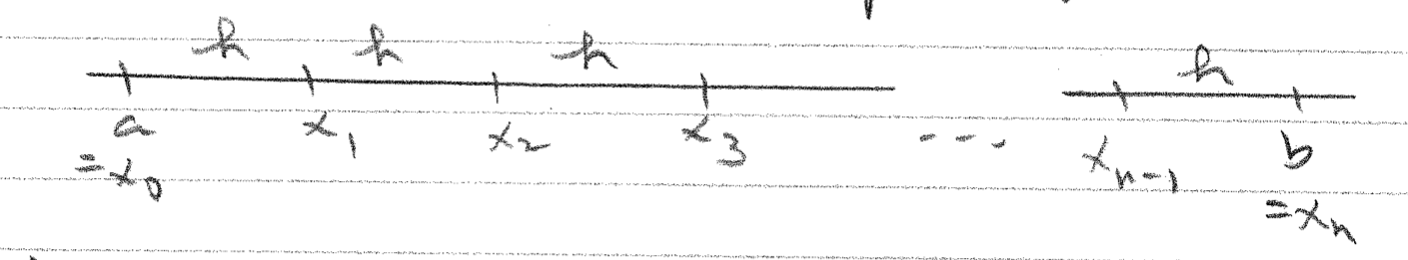
\includegraphics[scale=0.4]{linear_step_size}
  \label{fig:linear}
\end{figure}

\begin{align*} 
x_{i+1} - x_{i} = h, x_i = x_0 + ih 
\end{align*} 

If $P_n(x)$ interpolates $f(x)$ at $a=x_0, x_1, x_2, \dots, b=x_n$ 
and 
\[
\int_{a}^{b} f(x)dx \approx \int_{a}^{b} P_n(x)dx 
\]
\noindent 
then the resulting quadrature formula is called a {\bf Newton-Cotes} closed formula. 
\end{frame} 


\section{Newton-Cotes closed quadrature formulas} 

\begin{frame}{Introduction} 
The case $n=1$: 

\begin{figure} 
  \centering
  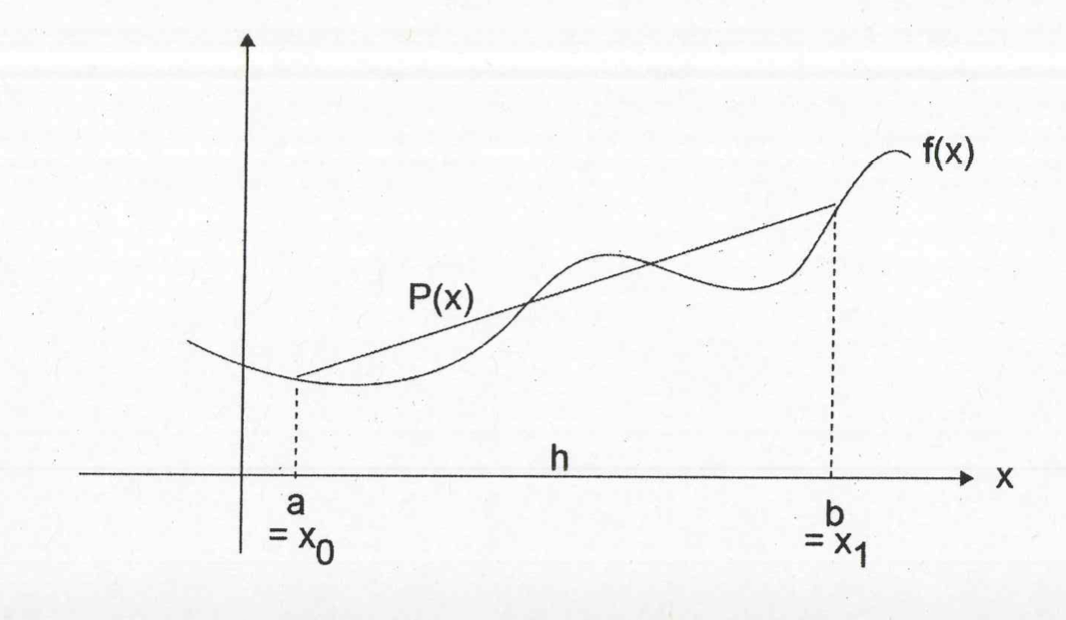
\includegraphics[scale=0.6]{linear_interpolating}
  \caption{Linear interpolating polynomial}
  \label{fig:linear}
\end{figure}
\noindent 
Here $h = b -a$. The (linear) interpolating polynomial is: 
\[
P(x) = \frac{x-x_1}{x_0-x_1}f(x_0) + \frac{x-x_0}{x_1-x_0} f(x_1) 
\]
\end{frame} 

\begin{frame}{Quadrature formula} 

The quadrature formula for approximating $\int_a^{b} f(x)dx$ is
obtained by integrating P(x):

\vspace{3 in}

\end{frame}

\begin{frame}{Quadrature formula continued} 


\end{frame}

\begin{frame}{Trapezoid rule}
This is the {\bf trapezoid rule}.
\[
\int_{a}^{b} f(x)dx \approx \frac{h}{2}[f(x_0)+f(x_1)]
\]
 Its error term can be obtained by
integrating the error term of the Lagrange form of the interpolating
polynomial, which for $n=1$ is
\[
f(x) - P(x) = \frac{f''(\xi)}{2}(x-x_0)(x-x_1) 
\]
\noindent 
where $\xi$ is in the interval $[a,b]$.
\end{frame}

\begin{frame}{Truncation Error} 
Integrating this gives: 

\begin{align*} 
\int_a^{b} f(x) dx - \int_{x_0}^{x_1} P(x)dx &= \int_a^{b} f(x) dx - \frac{h}{2} [ f(x_0) - f(x_1)] \\
&= \int_{a}^{b} \frac{f''(\xi)}{2}(x-x_0)(x-x_1)dx  \\
&= \frac{f''(\xi)}{2} \int_{a}^{b} (x-x_0)(x-x_1)dx \\ 
\end{align*} 

\noindent
since $f''(\xi)$ is a constant.

\end{frame} 


\begin{frame}{Truncation Error} 

Now, let $t = \frac{x-x_0}{h}$ and integrate $\frac{f''(\xi)}{2} \int_{a}^{b} (x-x_0)(x-x_1)dx$ by substitution of variables.
\vspace{3 in}

\end{frame} 

\begin{frame}{Truncation Error continued} 


\end{frame} 

\begin{frame}{Example 1}
Use the Trapezoidal Rule to numerically integrate \[f(x)=0.2+25x-200x^2+675x^3-900x^4+400x^5\] from $a=0$ to $b=0.8$ and approximate the absolute error.
\vspace{3 in}
\end{frame}

\begin{frame}{Example 1 continued}

\end{frame}

\begin{frame}{Qudratic case}

For the case $n=2$ the quadratic interpolating polynomial is: 

\begin{align*} 
P(x) &= \frac{(x-x_1)(x-x_2)}{(x_0-x_1)(x_0-x_2)}f(x_0)
+ \frac{(x-x_0)(x-x_2)}{(x_1-x_0)(x_1-x_2)}f(x_1) \\ 
& + \frac{(x-x_0)(x-x_1)}{(x_2-x_0)(x_2-x_1)}f(x_2)
\end{align*}
\begin{figure} 
  \centering
  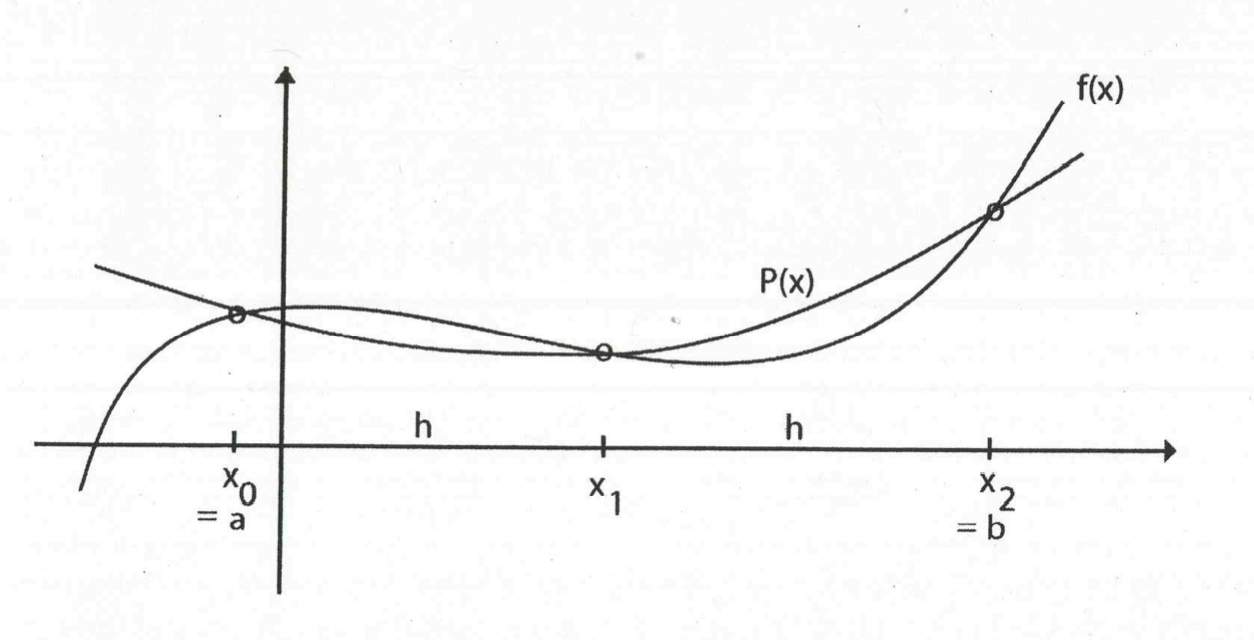
\includegraphics[scale=0.35]{quadratic_interpolating}
%  \caption{Quadratic interpolating polynomial}
  \label{fig:linear}
\end{figure}
\end{frame}


\begin{frame}{Qudrature formula for n=2} 
As in the case $n=1$, the quadrature formula for approximating $\int_a^{b} f(x)dx$ is obtained by integrating $P(x): \int_{a}^{b}f(x)dx \approx \int_{x_0}^{x_2}P(x)dx$. 

This gives: 
\[
   \int_{a}^{b} f(x)dx \approx \frac{h}{3}(f(x_0) + 4 f(x_1) + f(x_2))
\]
\noindent 
where now $h=\frac{b-a}{2}$. This is called {\bf Simpson's rule} or {\bf Simpson's 1/3 rule}, and its {\bf truncation error} is given by: 
\[
\int_{a}^{b}f(x)dx - \int_{x_0}^{x_2} P(x)dx = -\frac{h^5}{90} f^{(4)}(\xi), \mbox { for some } \xi \in [a,b] 
\]
\end{frame}

\begin{frame}{Example 2}
Use the Simpson's 1/3 Rule to numerically integrate \[f(x)=0.2+25x-200x^2+675x^3-900x^4+400x^5\] from $a=0$ to $b=0.8$ and approximate the absolute error.
\vspace{3 in}
\end{frame}

\begin{frame}{Example 2 continued}

\end{frame}

\begin{frame}{Quadrature formula for n=3} 

The Newton-Cotes closed quadrature formula for $n=3$ ({\bf Simpson's 3/8 rule}), in which $f(x)$
is approximated by a cubic polynomial that interpolates at four
equally-spaced points, is:
\[
\int_{a}^{b} f(x)dx \approx \frac{3h}{8} (f(x_0) + 3 f(x_1) + 3 f(x_2) + f(x_3)), 
\mbox { where } h = \frac{b-a}{3}
\]

The truncation error for this is
\[
E_t=\frac{-3}{80}h^5f^{(4)}(\xi)
\]
\noindent
for some $\xi \in [a,b]$.
\end{frame} 

\begin{frame}{Example 3}
Use the Simpson's 3/8 rule to numerically integrate \[f(x)=0.2+25x-200x^2+675x^3-900x^4+400x^5\] from $a=0$ to $b=0.8$ and approximate the absolute error.
\vspace{3 in}
\end{frame}

\begin{frame}{Example 3 continued}

\end{frame}
\section{Composite Newton-Cotes Formulas} 

\begin{frame}{Introduction} 
\begin{itemize}
\item{Corresponds to sections 21.1.2 and 21.2.2 of the text}
\item{{\bf Objective:} We want the {\bf truncation error $\rightarrow 0$} as the {\bf number of quadrature points $\rightarrow \infty$.}}
\item{Note: this does not happen in general as $n$, the order of the interpolating polynomial, $\rightarrow \infty$.}
\item{{\bf Solution:} We use composite (multiple-application) quadrature formulas.} 
\end{itemize}
\end{frame} 

\begin{frame}{Trapezoidal rule} 
\noindent 
Main idea: for $m \geq 1$, apply a closed N-C formula (with $n$ small) $m$ times on $[a,b]$. 

\noindent 
Example: Trapezoidal rule $(n=1)$ 
\\
For any $m \geq 1$, let $h = \frac{b-a}{m}$, subdivide $[a,b]$ into $m$ subintervals of length $h$, and apply the trapezoidal rule on each subinterval. 


\begin{figure}[h] 
  \centering
  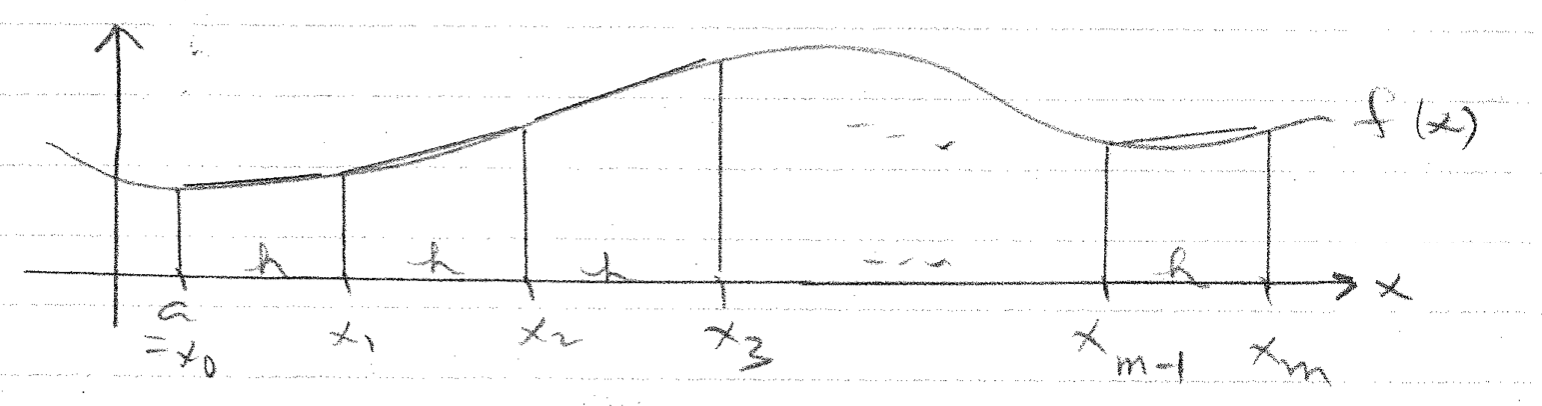
\includegraphics[scale=0.4]{composite_nc}
  \label{fig:composite_nc}
\end{figure}
\end{frame} 

\begin{frame}{Composite trapezoidal rule} 
\begin{align*} 
& \int_{a}^{b} f(x)dx = \int_{x_0}^{x_1}f(x)dx +  \int_{x_1}^{x_2}f(x)dx + \dots + \int_{x_{m-1}}^{x_m}f(x)dx \\ 
\approx & \int_{x_0}^{x_1}P_0(x)dx +  \int_{x_1}^{x_2}P_1(x)dx + \dots + \int_{x_{m-1}}^{x_m}P_{m-1}(x)dx \\
=& \frac{h}{2} \left [ f(x_0) + f(x_1) \right ] + \frac{h}{2} \left [ f(x_1) + f(x_2) \right ] + \dots + \frac{h}{2} \left [ f(x_{m-1}) + f(x_{m}) \right ] \\ 
=& h \left [ \frac{f(x_0)}{2} + \sum_{i=1}^{m-1} f(x_i) + \frac{f(x_m)}{2} \right ] 
\end{align*} 

This is called the composite trapezoial rule. 
\end{frame} 

\begin{frame}{Truncation Error}
\begin{align*} 
E_t =& -\frac{h^3}{12} f''(\xi_1) -\frac{h^3}{12} f''(\xi_2) - \dots - -\frac{h^3}{12} f''(\xi_m)  \\
=& -\frac{h^3}{12} \left [ f''(\xi_1) + f''(\xi_2) + \dots + f''(\xi_m) \right ] 
\end{align*} 
where $x_{i-1} \leq \xi_i \leq x_i$. 
\end{frame} 

\begin{frame}{Truncation Error II} 
We know that: 
\[
\min_{1 \leq i \leq m} f''(\xi_i) \leq \frac{f''(\xi_1) + f''(\xi_2) + \dots + f''(\xi_m)}{m} \leq \max_{1 \leq i \leq m} f''(\xi_i) 
\]

If $f''(x)$ is continuous on $[a,b]$, then there exists a value $\mu \in [a,b]$ such that: 

\[
f''(\mu) = \frac{f''(\xi_1) + f''(\xi_2) + \dots + f''(\xi_m)}{m} 
\]

This is called the intermediate value theorem. 

\[
E_t = - \frac{h^3}{12} [ m f''(\mu)] = - \frac{(b-a)}{12} h^2 f''(\mu) 
\]

since $h = \frac{b-a}{m}$. 
\end{frame} 

\begin{frame}{Example 1}
Let $m=2$ and apply the composite Trapezoid rule to numerically integrate the following function from $a=0$ to $b=0.8$.
\[
f(x)=0.2+25x-200x^2+675x^3-900x^4+400x^5
\]
\vspace{3 in}
\end{frame}

\begin{frame}{Example 1 continued}

\end{frame}

\begin{frame}{Important point} 

\[\lim_{m \rightarrow \infty} E_t = \lim_{h \rightarrow 0} E_t = 0
\]
provided that $f''(x)$ is continuous on $[a,b]$. 

\noindent 
(there is no comparable result as $n \rightarrow \infty$, where $n$ is the degree of the interpolating polynomial) 
\end{frame} 

\begin{frame}{Implementation} 
Usual implementation of composite trapezoidal: 
\begin{itemize} 
\item Initialize $m=1$ 
\item Repeatedly double $m$ (m=1,2,4,8,16,32,\dots )
\item Until two consecutive approximations are sufficiently close 
\end{itemize} 
\end{frame} 

\begin{frame}{Reusing function evaluations} 
The reason for using these values of $m$ is that they permit re-use of the function evaluations from previous evaluations

 i.e all values $f(x_i)$ computed for $m=k$ can be re-used for $m=2k$. 


\begin{figure}[h] 
  \centering
  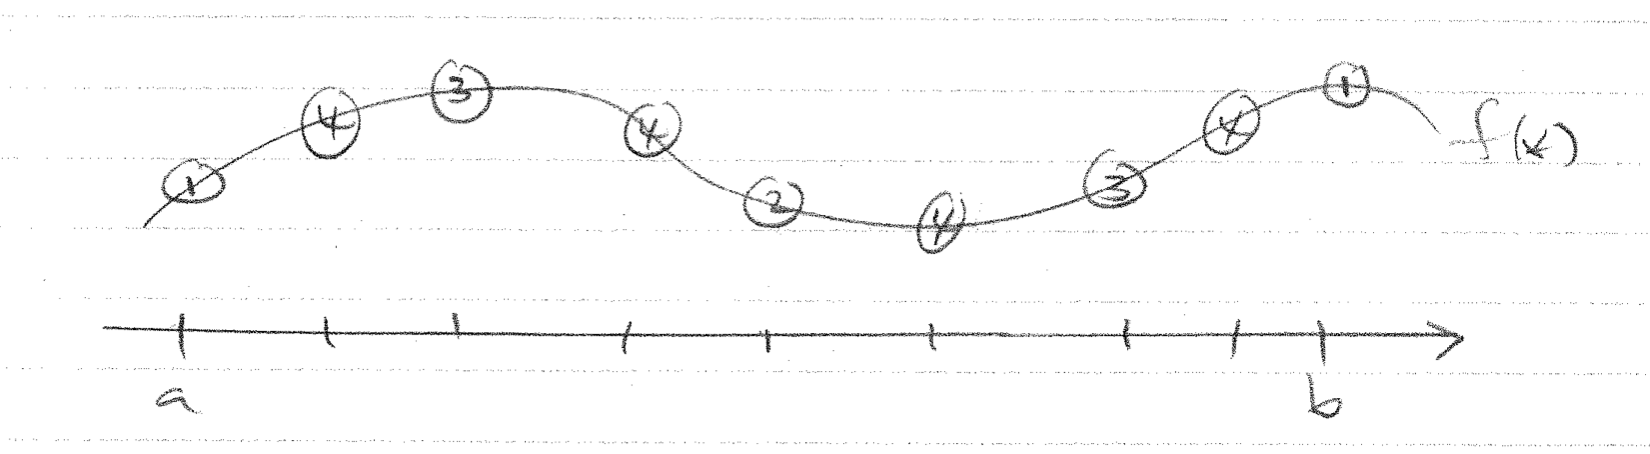
\includegraphics[scale=0.4]{reuse_of_points}
  \label{fig:reuse}
\end{figure}

\end{frame} 

\begin{frame}{Composite Simpson's Rule}
\begin{itemize}
\item{Each application of Simpson's rule requires 2 subintervals on the interval of integration and 3 quadrature points.}
\item{Thus, $m$ applications of Simpson's rule on $[a,b]$ require that $[a,b]$ be subdivided into $2m$ subintervals using $2m+1$ quadrature points.}
\item{Each subinterval then is of length
\[
h=\frac{b-a}{2m}
\]}
\end{itemize}
\vspace{2 in}
\end{frame}

\begin{frame}{Composite Simpson's Rule II}
Thus, at the $jth$ subinterval we have the three quadrature points $x_{2j-2}$, $x_{2j-1}$, and $x_{2j}$, and
\[
\int_{x_{2j-2}}^{x_{2j}} f(x)dx \approx \frac{h}{3} \left [ f(x_{2j-2}) + 4f(x_{2j-1}) + f(x_{2j}) \right ] 
\]			     

When $m=1$ (regular Simpson's rule) we have $2(1)+1=3$ quadrature points and 2 subintervals each of length $h=\frac{b-a}{2}$.
\vspace{2 in}
\end{frame}

\begin{frame}{Composite Simpson's Rule ($m=2$)}
When $m=2$, we apply Simpson's rule twice. We need $2(2)+1=5$ quadrature points to create $4$ subintervals each of length $h=\frac{b-a}{4}$.

\vspace{0.9 in}
Here,
\begin{align*} 
& \int_{a}^{b} f(x)dx \\
& \approx \frac{h}{3} \left [ f(x_0) + 4f(x_1) + f(x_2) \right ] + \frac{h}{3} \left [ f(x_2) + 4f(x_3) + f(x_4) \right ] \\
& = \frac{h}{3} \left [ f(x_0) + 4f(x_1) + 2f(x_2) + 4f(x_3) + f(x_4) \right ]
\end{align*} 


\end{frame}

\begin{frame}{General Composite Simpson's Rule}
In general, when $m \geq 1$, the composite Simpson's rule approximation is

\begin{multline*} 
 \int_{a}^{b} f(x)dx \\
 \approx \frac{h}{3}  [f(x_0) + 4f(x_1) + 2f(x_2) + 4f(x_3) + 2f(x_4) + \\ 
     \dotsm + 2f(x_{2m-2}) + 4f(x_{2m-1}) + f(x_{2m})]  \\
 = \frac{h}{3} \left [ f(x_0) + 4\sum_{j=1}^{m}f(x_{2j-1}) + 2\sum_{j=1}^{m-1}f(x_{2j}) + f(x_{2m}) \right ]
\end{multline*} 


\end{frame}

\begin{frame}{Truncation Error}
\begin{align*} 
E_t =& -\frac{h^5}{90} f^{(4)}(\xi_1) -\frac{h^5}{90} f^{(4)}(\xi_2) - \dots - -\frac{h^5}{90} f^{(4)}(\xi_m)  \\
=& -\frac{h^5}{90} \left [ f^{(4)}(\xi_1) + f^{(4)}(\xi_2) + \dots + f^{(4)}(\xi_m) \right ] \\
=& - \frac{h^5}{90} [ m f^{(4)}(\mu)]
\end{align*} 
where $a \leq \mu\leq b$ and $f^{(4)}(x)$ is continous. So,
\begin{align*} 
E_t = -\frac{(b-a)h^4}{180}f^{(4)}(\mu)
\end{align*} 
since $h = \frac{b-a}{2m}$. 
\end{frame} 

\begin{frame}{Example 2}
Let $m=2$ and apply the composite Simpson's rule to numerically integrate the following function from $a=0$ to $b=0.8$.
\[
f(x)=0.2+25x-200x^2+675x^3-900x^4+400x^5
\]
\vspace{3 in}
\end{frame}

\begin{frame}{Example 2 continued}

\end{frame}

\end{document} 



